\documentclass{article}
\usepackage[margin=0.5in]{geometry}
\usepackage{amsmath}
\usepackage{graphicx}
\usepackage{amssymb}
\usepackage{multicol}
\usepackage{xcolor}
\usepackage{amsthm}
\usepackage{mdframed}
\usepackage{tikz}
\usepackage [english]{babel}
\usepackage [autostyle, english = american]{csquotes}
\MakeOuterQuote{"}

\newcommand{\R}{\mathbb{R}}
\newcommand{\Z}{\mathbb{Z}}
\newcommand{\C}{\mathbb{C}}
\newcommand{\K}{\mathbb{K}}
\newcommand{\PP}{\mathbb{P}}
\newcommand{\E}{\mathcal{E}}
\newcommand{\e}{\vspace{3mm}}
\title{Práctica 1 - Experimentos aleatorios. Espacio muestral; eventos}
\author{Santiago}
\date{}
\begin{document}
    \maketitle
    \begin{enumerate}
        \item Asociar un espacio muestral a cada uno de los siguientes experimentos aleatorios.
    \begin{enumerate}
        \item Lanzar tres veces al aire una moneda y observar el lado que cae hacia arriba.
            \begin{mdframed}[style=s]
                El espacio muestral es el conjunto de resultados posibles de un experimento. En este caso particular, al tirar una moneda la misma puede caer con cara o cruz hacia arriba. Podemos denotar los siguientes eventos:
                \begin{center}
                    A: Sale cara\\
                    B: Sale cruz
                \end{center}
                Entonces tenemos que:\[\Omega=\{AAA,AAB,ABA,ABB,BAA,BBA,BAB,BBB\}\]
            \end{mdframed}
        \item Lanzar tres veces al aire una moneda y observar el número total de caras.
            \begin{mdframed}[style=s]
                Puede suceder que en los tres tiros no salga cara, también puede caer una vez, dos veces, e incluso tres. Por lo tanto:\[\Omega=\{0,1,2,3\}\]
            \end{mdframed}
        \item Una urna contiene 2 bolillas blancas y una negra. Se sacan 2 bolillas al azar simultáneamente y se anotan los colores.
            \begin{mdframed}[style=s]
                Como estoy anotando los colores, no se distingue entre las dos bolillas blancas. Considerando los eventos
                \begin{center}
                    N: negra\\
                    B: blanca
                \end{center}
                se tiene que\[\Omega=\{BB,BN\}\]
            \end{mdframed}
        \item Idem que en el inciso anterior pero con reemplazo.
            \begin{mdframed}[style=s]
                En este caso, al poder reemplazar, está la posibilidad de sacar dos veces la negra.\[\Omega=\{BB,BN,NN\}\]
                Hay que dintinguir entre sacar blanco-negro y negro-blanco?
            \end{mdframed}
        \item Se colocan al azar tres bolillas diferentes en tres urnas diferentes, pudiéndose poner más de una bolilla por urna.\vspace{3mm}\\
            Si representamos cada resultado como \[(U_{B_1},U_{B_2},U_{B_3})\]
            siendo $U_{B_i}$ la urna en donde se encuentra la bolilla $i$. Entonces
            \begin{center}
                $\Omega=\{(1,1,1),(1,1,2),(1,1,3),(1,2,1),(1,2,2),(1,2,3),(1,3,1),(1,3,2),(1,3,3),$\\
                $(2,1,1),(2,1,2),(2,1,3),(2,2,1),(2,2,2),(2,2,3),(2,3,1),(2,3,2),(2,3,3),$\\
                $(3,1,1),(3,1,2),(3,1,3),(3,2,1),(3,2,2),(3,2,3),(3,3,1),(3,3,2),(3,3,3)\}$
            \end{center}
            Como hay un número considerable de resultados, quizás es más conveniente expresar el espacio muestral por comprensión:
            \[\Omega=\{(i,j,k):i,j,k=1,2,3\}\]
        \item Se arroja una moneda; si sale cara se arroja un dado, si sale ceca se lanzan dos dados.\vspace{3mm}\\
            Si denominamos los siguientes eventos:
            \begin{center}
                A: cara\\
                B: ceca
            \end{center}
            \[\Omega=\{(A,i):i\in\mathbb{N}/i<7\}\cup\{(B,i,j):i,j=1,2,3,4,5,6\}\]
        \item Un viajante debe visitar cinco ciudades y traza su itinerario.\vspace{3mm}\\
            Supongamos que las ciudades las enumeramos del 1 al 5.\[\Omega=\{i_1,i_2,i_3,i_4,i_5:i_k\in[1;5],i_m\neq i_n\forall m\neq n\}\]
        \item Los artículos provenientes de una línea de producción se clasifican en defectuosos (D) y no defectuosos (N). Se observan artículos y se anota su condición. Este proceso se continúa hasta que se produzcan dos artículos defectuosos consecutivos o hasta que se hayan verificado cuatro artículos cualesquiera.
            \[\Omega=\{DD,NDD,NNDD,DNDD,DNDN,DNND,DNNN,NNNN,NDND,NDNN,NNDN,NNND\}\]
        \item Una caja con 12 lámparas tiene 4 unidades con filamentos rotos. Se las prueba hasta que se encuentre una
        quemada.\vspace{3mm}\\
            Definimos los eventos:
            \begin{center}
                Q: quemada\\
                N: no quemada
            \end{center}
            Entonces,
            \[\Omega=\{N^iQ:0\leq i\leq8\}\]
        \item Un tanque de agua tiene una bomba cuyo motor se pone en funcionamiento automáticamente cuando el consumo
        hace que el volumen de agua baje hasta cierto nivel. Supongamos que esto puede ocurrir a lo sumo una vez al
        día. Cierto día se observa el motor durante 24 horas y se registra en qué instante ha comenzado a funcionar o
        si no lo ha hecho en todo el día.\vspace{3mm}
            \begin{center}
                X: se prendió la bomba en el momento X\\
                N: no se prendió la bomba
            \end{center}
            Por lo tanto,
            \[\Omega=\{X,N\}\]
    \end{enumerate}
        \item Se examinan tres fusibles en secuencia, y se observa en cada caso si están o no defectuosos.
    \begin{enumerate}
        \item Describir el espacio muestral del experimento. ¿Cuántos elementos tiene?\vspace{3mm}\\
            Sean los eventos:
            \begin{center}
                D: defectuoso\\
                N: no defectuoso
            \end{center}
            Entonces se tiene que
            \[\Omega=\{DDD,DDN,DND,DNN,NDD,NDN,NND,NNN\}\]
            y se observa que
            \[\#\Omega=8\]
        \item Expresar por extensión los siguientes eventos:
            \begin{enumerate}
                \item $C:$ exactamente un fusible está defectuoso.
                    \[C=\{DNN,NDN,NND\}\]
                \item $D:$ a lo sumo un fusible está defectuoso.
                    \[D=C\cup\{NNN\}\]
                \item $E:$ los tres fusibles están en las mismas condiciones.
                    \[E=\{DDD,NNN\}\]
                \item ¿Cuáles de los sucesos $C,D$ o $E$ son mutuamente excluyentes?.\e\\
                    Se tiene que\[C\cap D=C\qquad C\cap E=\varnothing\qquad D\cap E=\{NNN\}\]
                    Por lo tanto, $C$ y $E$ son mutuamente excluyentes.\e
                \item Sean los eventos $A_i:$ el fusible $i-$ésimo está defectuoso $i=1,2,3$. Expresar los eventos anteriores en función de $A_1,A_2,A_3$.
                    \begin{center}
                        $C=\{A_1,A_2,A_3\}$\\
                        $D=C\cup\{A_1^cA_2^cA_3^c\}$\\
                        $E=\{A_1A_2A_3,A_1^cA_2^cA_3^c\}$
                    \end{center}\e
                \item Sean los eventos $B_i:$ hay exactamente $i$ fusibles defectuosos con $i=0,1,2,3$. ¿Cuántos elementos tiene cada $B_u$?
                    \begin{center}
                        $B_0=\{NNN\}\to \#B_0=1$\\
                        $B_1=\{NND,NDN,DNN\}\to\#B_1=3$\\
                        $B_2=\{NDD,DDN,DND\}\to\#B_2=3$\\
                        $B_3=\{DDD\}\to\#B_3=1$
                    \end{center}
            \end{enumerate}
    \end{enumerate}
        \item Una instalación consta de dos calderas y un motor. Sea $M$ el evento de que el motor está en buenas condiciones, mientras que los sucesos $C_i(i=1,2)$ son los eventos de que la $i-$ésima caldera está en buenas condiciones. El evento $I$ es que la instalación funcione. Si la instalación funciona cada vez que el motor y al menos una caldera están en buenas condiciones, exprese $I$ e $I^c$ mediante $M,C_1$ y $C_2$.
    \[I=\{MC_1C_2,MC_1^cC_2,MC_1C_2^c\}\qquad I^c=\{MC_1^cC_2^c,M^cC_1^cC_2^c,M^cC_1^cC_2,M^cC_1C_2^c,M^cC_1C_2\}\]
        \item Se arrojan dos dados. Sean $E=$"la suma de los números obtenidos es impar", $F=$"sale el 1 al menos una vez", $G=$"la suma es 5". Descubrir los eventos:
    \begin{enumerate}
        \item $E\cap F$\e\\
            Primero se escriben los eventos mencionados:
            \begin{center}
                $E=\{12,14,16,21,23,25,32,34,36,41,43,45,52,54,56,61,63,65\}$\\
                $F=\{11,12,13,14,15,16,21,31,41,51,61\}$\\
                $G=\{14,23,32,41\}$
            \end{center}
            Entonces,
            \[E\cap F=\{12,14,16,21,41,61\}\]
        \item $E\cup F$
            \[E\cup F=\{12,14,16,21,23,25,32,34,36,41,43,45,52,54,56,61,63,65,11,13,15,31,51\}\]
        \item $E\cap F^c$
            \[E\cap F^c=\{23,25,32,34,36,43,45,52,54,56,63,65\}\]
        \item $F\cap G$
            \[F\cap G=\{14,41\}\]
        \item $E\cap F\cap G$
            \[E\cap F\cap G=\{14,41\}\]
    \end{enumerate}
        \item Se realiza el siguiente experimento aleatorio: se lanza una moneda y un dado.
    \begin{enumerate}
        \item Definir un espacio muestral.\e\\
            La moneda puede resultar en cara o ceca, mientras que el dado en un natural menor o igual a 6.
            \begin{center}
                $X=$ cara\\
                $Y=$ ceca\\
            \end{center}
            Por lo tanto, el espacio muestral resulta ser\[\Omega=\{X1,X2,X3,X4,X5,X6,Y1,Y2,Y3,Y4,Y5,Y6\}\]
        \item Expresar explícitamente los siguientes sucesos:\\
            $A=$ "se obtiene un par y una cara".
            \[A=\{X2,X4,X6\}\]
            $B=$ "se obtiene un número primo".
            \[B=\{X2,X3,X5,Y2,Y3,Y5\}\]
            $C=$ "se obtiene un número impar y una ceca".
            \[C=\{Y1,Y3,Y5\}\]
        \item Encontrar expresiones para los siguientes eventos:
            \begin{enumerate}
                \item Sólamente ocurre $B$.\e\\
                    "Se obtiene un número primo"\e
                \item Ocurren tanto $A$ como $B$ pero no ocurre $C$.\e\\
                    "Se obtiene cara y un dos"\e
                \item Por lo menos dos ocurren.
                \item Ocurre uno y no más.
                \item No ocurren más de dos.
            \end{enumerate}
    \end{enumerate}
        \item En un estudio realizado con 900 profesionales, 25 años después de su graduación, se descubre que 300 de ellos tuvieron éxito profesional, 300 de ellos se radicaron en el extranjero y 100 de ellos tuvieron éxito y se radicaron en el extranjero. Hallar el número de personas en el grupo que de estas dos cosas hayan hecho:
    \begin{enumerate}
        \item exactamente dos.\e\\
            Si se consideran los eventos
            \begin{center}
                $A=$ es exitoso\\
                $B=$ radicado en el extranjero 
            \end{center}
            es posible realizar el siguiente diagrama de Venn
            \begin{center}
                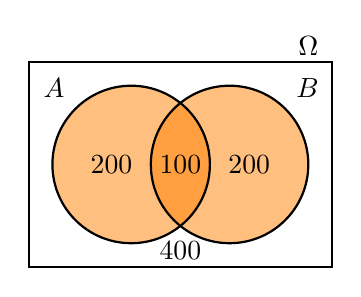
\begin{tikzpicture}[thick,
                    set/.style = {circle,
                                minimum size = 2cm,
                                fill=orange,
                                opacity=0.5}]
                    \draw [draw=black] (-1.3,-1.3) rectangle (2.55,1.3);
                    % Set A
                    \node[set,label={135:$A$}] (A) at (0,0) {};
                    % Set B
                    \node[set,label={45:$B$}] (B) at (1.25,0) {};
                    % Circles outline
                    \draw (0,0) circle(1cm);
                    \draw (1.25,0) circle(1cm);
                    % Set intersection label
                    \node at (0.625,0) {100};
                    \node at (-0.25,0) {200};
                    \node at (1.5,0) {200};
                    \node at (0.625,-1.1) {400};
                    \node at (2.25,1.5) {$\Omega$};
                \end{tikzpicture}
            \end{center}
            Hay 100 personas que son exitosas y están radicadas en el extranjero
        \item por lo menos una.\e\\
            En el diagrama podemos ver que hay 400 personas que no lograron ninguna de las dos, así que son $500(=900-400)$ aquellas que al menos lograron una.\e
        \item no más de una.\e\\
            Este grupo está conformado por las 200 personas que son exitosas pero no están en el extranjero y por las 200 personas radicadas en el extranjero pero no exitosas. Por lo tanto, hay 400 personas en total.
    \end{enumerate}
        \item Un experimento aleatorio tiene tres resultados posibles: $a,b$ y $c$, con probabilidades $p,p^2$ y $p$ respectivamente. Hallar justificando apropiadamente el/los valores válidos de $p$.\e\\
    Tenemos que el espacio muestral es\[\Omega=\{a,b,c\}\]
    Entonces, por axioma 3:\begin{align*}
        P(\Omega)=1&=p(a)+p(b)+p(c)=p+p^2+p\\
        &\to p^2+2p-1=0\\
        &\to p=-1\pm\sqrt{2} 
    \end{align*}
    Sin embargo, $-1-\sqrt{2}$ implica una probabilidad negativa con lo cual\[p=-1+\sqrt{2}\]
        \item Una caja tiene 10 bolas numeradas del 1 al 10. Una bola se elige al azar y una segunda bola se elige de las 9 restantes. Encontrar la probabilidad de que los números de las 2 bolas difieran en 2 o más.\e\\
    La primera bola puede ser cualquiera de las 10 en la caja mientras que la segunda es una entre nueve, por ende, hay \[10\cdot9=90\text{ casos totales}\]
    Para determinar los casos favorables, se puede pensar de la siguiente forma: Si saco 1 o 10, tengo 8 bolas que cumplen lo pedido
    \begin{center}
        $B_1=1\to B_2=i,\quad i=3,4,5,6,7,8,9,10$\\
        $B_1=10\to B_2=j,\quad j=1,2,3,4,5,6,7,8$ 
    \end{center}
    Mientras que con los otros números sólo tengo 7 opciones favorables ya que su anterior y siguiente no son válidos. Ej:\[B_1=5\to B_2=k,\quad k=1,2,3,7,8,9,10\]
    Teniendo en cuenta esto hay\[8\cdot7+2\cdot8=72\text{ casos favorables}\]
    Por lo tanto, sea $A=$ las bolas difieren en 2 o más, se tiene que\[P(A)=\frac{72}{90}\]
    También se podría haber pensado que\[P(A)=1-P(A^c)\]
    En donde $A^c$ contempla los casos en donde las bolas difieren en 1. Nuevamente, hay que separar de la siguiente manera: Si saco 1 o 10, la siguiente debe ser 2 o 9 respectivamente, para el resto hay 2 opciones. Entonces,
    \[P(A)=1-\frac{2\cdot1+8\cdot2}{90}=1-\frac{18}{90}=\frac{72}{90}\]
        \item Se carga un dado de manera que los números pares tienen el doble de probabilidad de salir que los impares; los pares son igualmente probables entre sí, y lo mismo sucede con los impares. Se arroja el dado una vez. Hallar la probabilidad que:
    \begin{enumerate}
        \item Aparezca un número par.\e\\
            Tenemos que los impares son la mitad de probables que los pares. Si consideramos los eventos
            \begin{center}
                $A=$ sale un número par\\
                $B=$ sale un número impar
            \end{center}
            Entonces\[P(A)=2P(B)\]
            Además, el espacio muestral es\[\Omega=\{1,2,3,4,5,6\}\]
            y se sabe que\[A=\{2,4,6\}\qquad B=\{1,3,5\}\]
            Por el axioma 3\[P(A)=p(2)+p(4)+p(6)\qquad P(B)=p(1)+p(3)+p(5)\]
            Y como cada par e impar tienen la misma probabilidad entre sí\[P(A)=6c\qquad P(B)=3c\]
            Al ser $A$ y $B$ disjuntos, por la propiedad 1\[P(\Omega)=P(A\cup B)=P(A)+P(B)=9c=1\to c=\frac{1}{9}\]
            Por lo tanto\[P(A)=6\cdot\frac{1}{9}=\frac{6}{9}\]
        \item Aparezca un número impar.
            \[P(B)=3\cdot\frac{1}{9}=\frac{3}{9}\]
        \item Aparezca un número primo impar.\e\\
            Los números primos impares que pueden salir en un dado son 3 y 5. Como los impares son igual de probables y $P(B)=\frac{3}{9}\to p(1)=p(3)=p(5)=\frac{1}{9}$\[\to p(3)+p(5)=\frac{2}{9}\]
    \end{enumerate}
        \item Sean $A$ y $B$ dos eventos tales que $P(A)=0.5,P(A\cap B)=0.2$ y $P(A\cup B)=0.7$. Hallar
    \begin{enumerate}
        \item $P(B)$\e\\
            Del principio de inclusión-exclusión se sabe que $P(A\cup B)=P(A)+P(B)-P(A\cap B)$. Entonces,\begin{center}
                $P(B)=P(A\cup B)+P(A\cap B)-P(A)$\\
                $\to P(B)=0.7+0.2-0.5$\\
                $\to P(B)=0.4$    
            \end{center}
        \item $P$(ocurra exactamente uno de los dos eventos)\e\\
            La probabilidad de que suceda alguno de los dos eventos está dada por $P(A\cup B)$. A ésta hay que restarle la probabilidad de que sucedan los dos simultáneamente, Entonces\[P(\text{ocurra exactamente uno de los dos eventos})=P(A\cup B)-P(A\cap B)=0.5\]
        \item $P$(no ocurra ninguno de los eventos)\e\\
            Se sabe que la probabilidad de que ocurra al menos uno es $P(A\cup B)$. Entonces\[P(\text{no ocurra ninguna de los eventos})=1-P(A\cup B)=0.3\]
    \end{enumerate}
        \item Sean $A$ y $B$ dos eventos. Suponiendo que $P(A)=x,P(B)=y,P(A\cap B)=z$. Expresar cada una de las siguientes probabilidades en términos de $x,y,z$.
    \begin{enumerate}
        \item $P(A^c\cap B^c)$
            \begin{align*}
                P(A^c\cap B^c)&=P((A\cup B)^c)&&\text{De Morgan}\\
                &=1-P(A\cup B)&&\text{Propiedad 2}\\
                &=1-(P(A)+P(B)-P(A\cap B))&&\text{Propiedad 5}\\
                &=1-(x+y-z)&&\text{Definición}\\
                P(A^c\cap B^c)&=1-x-y+z
            \end{align*}
        \item $P(A^c\cap B)$
            \begin{align*}
                P(A^c\cap B)&=P((A^c\cap B) \cup\varnothing)\\
                &=P((A^c\cap B)\cup(B\cap B^c))\\
                &=P(B\cap(A^c\cup B^c))&&\text{Distributiva}\\
                &=P(B\cap(A\cap B)^c)&&\text{De Morgan}\\
                &=P(B-(A\cap B))&&\text{Def Resta}\\
                &=P(B)-P(A\cap B)&&\text{Propiedad 3}\\
                &=y-z
            \end{align*}
        \item $P(A^c\cup B^c)$
            \begin{align*}
                P(A^c\cup B^c)&=P((A\cap B)^c)&&\text{De Morgan}\\
                &=1-P(A\cap B)&&\text{Propiedad 2}\\
                &=1-z
            \end{align*}
        \item $P(\text{ocurra al menos uno de los dos eventos})$
            \begin{align*}
                &=P(A\cup B)\\
                &=P(A)+P(B)-P(A\cap B)&&\text{Propiedad 5}\\
                &=x+y-z
            \end{align*}
        \item $P(\text{ocurra a lo sumo uno de los dos eventos})$
            \begin{align*}
                &=1-P(A\cap B)\\
                &=1-z
            \end{align*}
    \end{enumerate}
        \item Durante  un año las personas de una ciudad utilizan tres tipos de transportes: metro (M), autobús (A) y coche particular (C). Las probabilidades de que durante el año hayan usado unos u otros transportes son las siguientes: sólo metro = 0,30; sólo autobús = 0,20; sólo coche = 0,15; sólo metro y autobús = 0,10; sólo metro y coche = 0,05; sólo autobús y coche = 0,06; metro,autobús y coche = 0,01.\\
    Calcular las siguientes probabilidades:
    \begin{enumerate}
        \item Que una persona tome al menos dos medios de transporte.\e\\
            $B=$ "la persona toma al menos dos medios de transporte"\\
            $B_{MA}=$ "la persona toma sólo metro y autobús"\\
            $B_{MC}=$ "la persona toma sólo metro y coche"\\
            $B_{AC}=$ "la persona toma sólo autobús y coche"\\
            $B_{T}=$ "la persona toma todos los medios de transporte"\\
            Entonces tenemos que\[P(B)=P(B_{MA}\cup B_{MC}\cup B_{AC}\cup B_{T})\]
            Como los eventos son mutuamente excluyentes\begin{align*}
                P(B)&=P(B_{MA})+P(B_{MC})+P(B_{AC})+P(B_{T})\\
                &=0,10+0,05+0,06+0,01\\
                &=0,22
            \end{align*}
        \item Que una persona viaje en metro y no en autobús.\e\\
            $M=$ "la persona viaja en metro"\\
            $A=$ "la persona viaja en autobús"\\
            Me interesa calcular $P(M-A)=P(M-(M\cap A))=P(M)-P(M\cap A)$ debido a que $M\cap A \subset M$
            \begin{align*}
                P(M)-P(M\cap A)&=[P(\text{sólo en metro})+P(B_{MA})+P(B_{MC})+P(T)]-[P(B_{MA})+P(T)]\\
                &=P(\text{sólo en metro})+P(B_{MC})\\
                &=0,35
            \end{align*}
        \item Que una persona viaje en metro o en coche y no en autobús.\e\\
            $C=$ "la persona viaja en coche"
            \begin{align*}
                P((M\cup C)-A)&=P((M\cup C)-((M\cup C)\cap A))\\
                &=P(M\cup C)-P((M\cup C)\cap A)\\
                &=P(M)+P(C)-P(M\cap C)-P(M\cap A\cup C\cap A)\\
                &=P(M)+P(C)-P(M\cap C)-P(M\cap A)-P(C\cap A)+P(M\cap A\cap C)\\
                &=P(M)+P(C)-[P(B_{MC})+P(T)]-[P(B_{MA})+P(T)]-[P(B_{CA}+P(T))]+P(T)\\
                &=P(M)+P(C)-P(B_{MC})-P(B_{MA})-P(B_{CA})-2P(T)
            \end{align*}
            Tenemos que \begin{align*}
                P(M)=P(\text{sólo en metro})+P(B_{MA})+P(B_{MC})+P(T)=0,3+0,1+0,05+0,01=0,46\\
                P(C)=P(\text{sólo en coche})+P(B_{CA})+P(B_{MC})+P(T)=0,15+0,06+0,05+0,01=0,27
            \end{align*}
            Entonces,\begin{align*}
                P((M\cup C)-A)&=0,46+0,27-0,05-0,1-0,06-2\cdot0,01\\
                &=0,5
            \end{align*}
        \item Que viaje en metro o en autobús y en coche.
            \begin{align*}
                P((M\cup A)\cap C)&=P(M\cap C\cup A\cap C)\\
                &=P(M\cap C)+P(A\cap C)-P(M\cap C\cap A)\\
                &=P(B_{MC})+P(T)+P(B_{AC})+P(T)-P(T)\\
                &=P(B_{MC})+P(B_{AC})+P(T)\\
                &=0,05+0,06+0,01\\
                &=0,12
            \end{align*}
        \item Que una persona vaya a pie.\e\\
            $E=$ "la persona va a pie"\\
            $E^c=$ "la persona toma algún transporte" 
            Se sabe que \[P(E)=1-P(E^c)\]
            En donde \begin{align*}
                P(E^c)&=P(M\cup A\cup C)\\
                &=P(M)+P(A)+P(C)-P(MA)-P(MC)-P(AC)+P(AMC)\\
                &=P(M)+P(A)+P(C)-P(B_{MA})-P(T)-P(B_{MC})-P(T)-P(B_{AC})-P(T)+P(T)\\
                &=P(M)+P(A)+P(C)-P(B_{MA})-P(B_{MC})-P(B_{AC})-2P(T)\\
            \end{align*}
            Se tiene que $P(A)=P(\text{sólo en autobús})+P(B_{MA})+P(B_{CA})+P(T)=0,37$. Entonces,
            \[P(E^c)=0,46+0,37+0,27-0,1-0,05-0,06-2\cdot0,01=0,87\]
            Por lo tanto \[P(E)=1-0,87=0,13\]
            También se podría haber hecho un diagrama de Venn y analizar cada situación como sigue
            \begin{enumerate}
                \item La persona toma al menos dos medios de transporte\e\\
                    Si toma al menos dos, el sector de interés es
                    \begin{center}
                        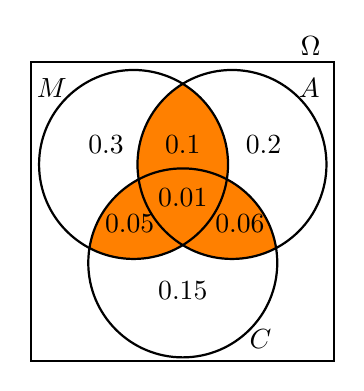
\begin{tikzpicture}
                            [thick,
                            set/.style = {circle,
                                        minimum size = 2cm}]
                            \fill[white] (-1.3,-2.5) rectangle (2.55,1.3);
                            \begin{scope}
                                \clip (1.25,0) circle (1.2);
                                \clip (0,0) circle (1.2);
                                \fill[orange] (-1.3,-2.5) rectangle (2.55,1.3);
                            \end{scope}
                            \begin{scope}
                                \clip (1.25,0) circle (1.2);
                                \clip (0.625,-1.25) circle (1.2);
                                \fill[orange] (-1.3,-2.5) rectangle (2.55,1.3);
                            \end{scope}
                            \begin{scope}
                                \clip (0,0) circle (1.2);
                                \clip (0.625,-1.25) circle (1.2);
                                \fill[orange] (-1.3,-2.5) rectangle (2.55,1.3);
                            \end{scope}
                            \draw [draw=black] (-1.3,-2.5) rectangle (2.55,1.3);
                            % Conjunto Metro
                            \node[set,label={135:$M$}] (M) at (0,0) {};
                            % Conjunto autobús
                            \node[set,label={45:$A$}] (A) at (1.25,0) {};
                            % Conjunto coche
                            \node[set,label={315:$C$}] (C) at (0.625,-1.25) {};
                            % Dibujo conjuntos
                            \draw (0,0) circle(1.2cm);
                            \draw (1.25,0) circle(1.2cm);
                            \draw (0.625,-1.25) circle(1.2cm);
                            % Set intersection label
                            \node at (-0.35,0.25) {0.3};
                            \node at (1.65,0.25) {0.2};
                            \node at (0.625,0.25) {0.1};
                            \node at (0.625,-1.6) {0.15};
                            \node at (barycentric cs:A=1,M=1,C=1) {0.01};
                            \node at (-0.05,-0.75) {0.05};
                            \node at (1.35,-0.75) {0.06};
                            \node at (2.25,1.5) {$\Omega$};
                        \end{tikzpicture}
                    \end{center}
                    Con lo cual\[P(\text{al menos dos transportes})=0,1+0,01+0,05+0,06=0,22\]
                \item Viaje en metro y no en autobús
                    \begin{center}
                        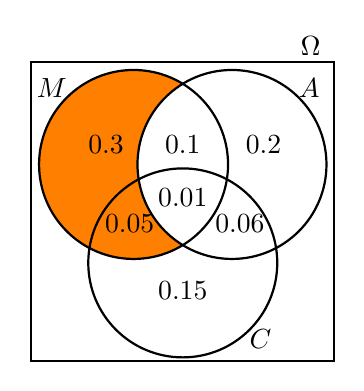
\begin{tikzpicture}
                            [thick,
                            set/.style = {circle,
                                        minimum size = 2cm}]
                            \fill[orange] (0,0) circle (1.2);
                            \begin{scope}
                                \clip (1.25,0) circle (1.2);
                                \clip (0,0) circle (1.2);
                                \fill[white] (0,0) circle (1.2);
                            \end{scope}
                            \draw [draw=black] (-1.3,-2.5) rectangle (2.55,1.3);
                            % Conjunto Metro
                            \node[set,label={135:$M$}] (M) at (0,0) {};
                            % Conjunto autobús
                            \node[set,label={45:$A$}] (A) at (1.25,0) {};
                            % Conjunto coche
                            \node[set,label={315:$C$}] (C) at (0.625,-1.25) {};
                            % Dibujo conjuntos
                            \draw (0,0) circle(1.2cm);
                            \draw (1.25,0) circle(1.2cm);
                            \draw (0.625,-1.25) circle(1.2cm);
                            % Set intersection label
                            \node at (-0.35,0.25) {0.3};
                            \node at (1.65,0.25) {0.2};
                            \node at (0.625,0.25) {0.1};
                            \node at (0.625,-1.6) {0.15};
                            \node at (barycentric cs:A=1,M=1,C=1) {0.01};
                            \node at (-0.05,-0.75) {0.05};
                            \node at (1.35,-0.75) {0.06};
                            \node at (2.25,1.5) {$\Omega$};
                        \end{tikzpicture}
                    \end{center}
                    De donde se sigue que\[P(\text{metro y no autobús})=0,3+0,05=0,35\]
                \item Metro o coche y no autobús
                    \begin{center}
                        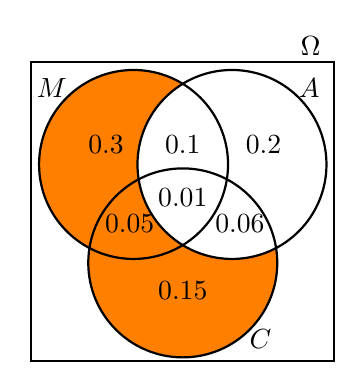
\begin{tikzpicture}
                            [thick,
                            set/.style = {circle,
                                        minimum size = 2cm}]
                            \fill[orange] (0,0) circle (1.2);
                            \begin{scope}
                                \clip (1.25,0) circle (1.2);
                                \clip (0,0) circle (1.2);
                                \fill[white] (0,0) circle (1.2);
                            \end{scope}
                            \fill[orange] (0.625,-1.25) circle (1.2);
                            \begin{scope}
                                \clip (1.25,0) circle (1.2);
                                \clip (0.625,-1.25) circle (1.2);
                                \fill[white] (1.25,0) circle (1.2);
                            \end{scope}
                            \draw [draw=black] (-1.3,-2.5) rectangle (2.55,1.3);
                            % Conjunto Metro
                            \node[set,label={135:$M$}] (M) at (0,0) {};
                            % Conjunto autobús
                            \node[set,label={45:$A$}] (A) at (1.25,0) {};
                            % Conjunto coche
                            \node[set,label={315:$C$}] (C) at (0.625,-1.25) {};
                            % Dibujo conjuntos
                            \draw (0,0) circle(1.2cm);
                            \draw (1.25,0) circle(1.2cm);
                            \draw (0.625,-1.25) circle(1.2cm);
                            % Set intersection label
                            \node at (-0.35,0.25) {0.3};
                            \node at (1.65,0.25) {0.2};
                            \node at (0.625,0.25) {0.1};
                            \node at (0.625,-1.6) {0.15};
                            \node at (barycentric cs:A=1,M=1,C=1) {0.01};
                            \node at (-0.05,-0.75) {0.05};
                            \node at (1.35,-0.75) {0.06};
                            \node at (2.25,1.5) {$\Omega$};
                        \end{tikzpicture}
                    \end{center}
                    Por ende\[P(\text{metro o coche y no autobús})=0,3+0,05+0,15=0,5\]
                \item Metro o autobús y coche.
                    \begin{center}
                        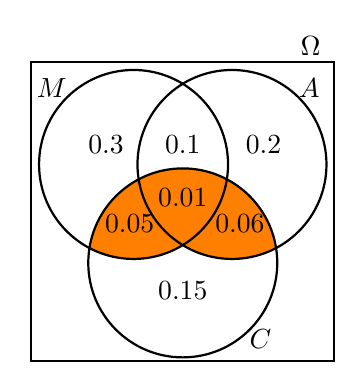
\begin{tikzpicture}
                            [thick,
                            set/.style = {circle,
                                        minimum size = 2cm}]
                            \fill[white] (0.625,-1.25) circle (1.2);
                            \begin{scope}
                                \clip (1.25,0) circle (1.2);
                                \clip (0.625,-1.25) circle (1.2);
                                \fill[orange] (1.25,0) circle (1.2);
                            \end{scope}
                            \begin{scope}
                                \clip (0,0) circle (1.2);
                                \clip (0.625,-1.25) circle (1.2);
                                \fill[orange] (0.625,-1.25) circle (1.2);
                            \end{scope}
                            \draw [draw=black] (-1.3,-2.5) rectangle (2.55,1.3);
                            % Conjunto Metro
                            \node[set,label={135:$M$}] (M) at (0,0) {};
                            % Conjunto autobús
                            \node[set,label={45:$A$}] (A) at (1.25,0) {};
                            % Conjunto coche
                            \node[set,label={315:$C$}] (C) at (0.625,-1.25) {};
                            % Dibujo conjuntos
                            \draw (0,0) circle(1.2cm);
                            \draw (1.25,0) circle(1.2cm);
                            \draw (0.625,-1.25) circle(1.2cm);
                            % Set intersection label
                            \node at (-0.35,0.25) {0.3};
                            \node at (1.65,0.25) {0.2};
                            \node at (0.625,0.25) {0.1};
                            \node at (0.625,-1.6) {0.15};
                            \node at (barycentric cs:A=1,M=1,C=1) {0.01};
                            \node at (-0.05,-0.75) {0.05};
                            \node at (1.35,-0.75) {0.06};
                            \node at (2.25,1.5) {$\Omega$};
                        \end{tikzpicture}
                    \end{center}
                    \[P(\text{metro o autobús y coche})=0,05+0,01+0,06=0,12\]
                \item Que vaya a pie.
                \begin{center}
                    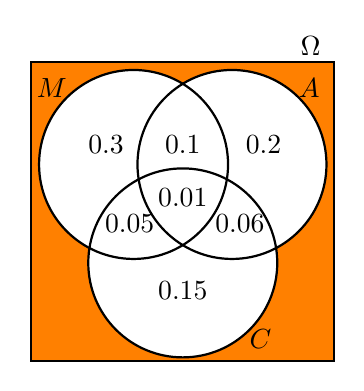
\begin{tikzpicture}
                        [thick,
                        set/.style = {circle,
                                    minimum size = 2cm}]
                        \fill[orange] (-1.3,-2.5) rectangle (2.55,1.3);
                        \begin{scope}
                            \clip (1.25,0) circle (1.2);
                            \fill[white] (1.25,0) circle (1.2);
                        \end{scope}
                        \begin{scope}
                            \clip (0.625,-1.25) circle (1.2);
                            \fill[white] (0.625,-1.25) circle (1.2);
                        \end{scope}
                        \begin{scope}
                            \clip (0,0) circle (1.2);
                            \fill[white] (0,0) circle (1.2);
                        \end{scope}
                        \draw [draw=black] (-1.3,-2.5) rectangle (2.55,1.3);
                        % Conjunto Metro
                        \node[set,label={135:$M$}] (M) at (0,0) {};
                        % Conjunto autobús
                        \node[set,label={45:$A$}] (A) at (1.25,0) {};
                        % Conjunto coche
                        \node[set,label={315:$C$}] (C) at (0.625,-1.25) {};
                        % Dibujo conjuntos
                        \draw (0,0) circle(1.2cm);
                        \draw (1.25,0) circle(1.2cm);
                        \draw (0.625,-1.25) circle(1.2cm);
                        % Set intersection label
                        \node at (-0.35,0.25) {0.3};
                        \node at (1.65,0.25) {0.2};
                        \node at (0.625,0.25) {0.1};
                        \node at (0.625,-1.6) {0.15};
                        \node at (barycentric cs:A=1,M=1,C=1) {0.01};
                        \node at (-0.05,-0.75) {0.05};
                        \node at (1.35,-0.75) {0.06};
                        \node at (2.25,1.5) {$\Omega$};
                    \end{tikzpicture}
                \end{center}
                \[P(\text{vaya a pie})=1-(0,3+0,1+0,2+0,05+0,01+0,06+0,15)=0,13\]
            \end{enumerate}
    \end{enumerate}
        \item Se selecciona un punto al azar en el interior de un círculo. Hallar la probabilidad de que el punto quede más cercano al centro que a la circunferencia.\e\\
    Se tiene la siguiente situación
    \begin{center}
        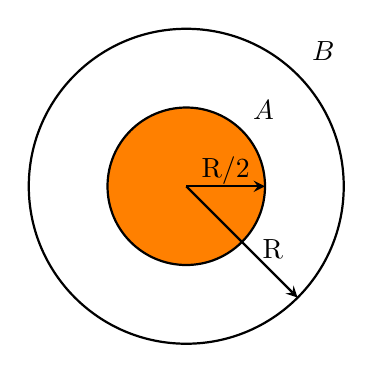
\begin{tikzpicture}
            [thick,
            set/.style = {circle,
                        minimum size = 2cm}]
            \fill[orange] (0,0) circle (1);
            \node[set,label={45:$A$}] (A) at (0,0) {};
            \node[set,label={45:$B$}] (B) at (0.75,0.75) {};
            % Dibujo conjuntos
            \draw (0,0) circle(1cm);
            \draw (0,0) circle(2cm);
            \draw [-stealth](0,0) -- (1,0);
            \draw [-stealth](0,0) -- (1.414,-1.414);

            \node at (0.5,0.2) {R/2};
            \node at (1.1,-0.8) {R};
        \end{tikzpicture}
    \end{center}
    En donde A es el área de interés, mientras que B es el área total. Entonces,
    \[P(A)=\frac{\text{área }A}{\text{área }B}=\frac{\pi \cdot (R/2)^2}{\pi\cdot R^2}=\frac{1}{4}\]
        \item Se escoge al azar un punto $X$ sobre un segmento de recta $AB$ con punto medio $O$. Hallar la probabilidad de que los segmentos de recta $AX,XB$ y $AO$ puedan formar un triángulo. (Recordar la propiedad triangular: \textit{En todo triángulo un lado es menor que la suma de los otros dos y mayor que su diferencia}).
    \begin{center}
        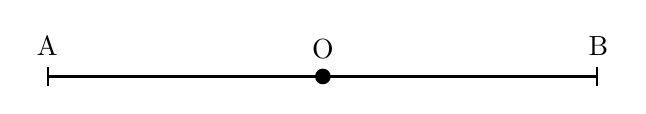
\begin{tikzpicture}[mynode/.style={fill,circle,inner sep=2pt,outer sep=0pt}
            ]
            \draw[thick] [|-|] (0,0) -- (7,0)
            node[pos=0,label=above:{A}]{}
            node[pos=0.5,mynode,label=above:{O}]{}
            node[pos=1,label=above:{B}]{};
        \end{tikzpicture}
    \end{center}
    Se tiene que\[AX+XB=AB\qquad AO=AB/2\]
    De la propiedad triangular:\begin{align*}
        AX<XB+AO\to AX<AB-AX+AB/2\to AX<\tfrac{3}{4}AB\\
        AX>XB-XO\to AX>AB-AX-AB/2\to AX>\tfrac{1}{4}AB
    \end{align*}
    Entonces tenemos que el intervalo válido para $X$ es el naranja:
    \begin{center}
        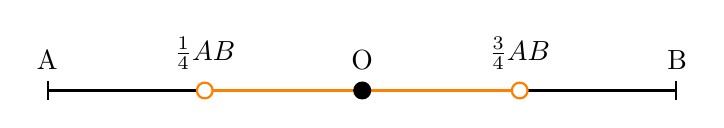
\begin{tikzpicture}
            \draw[thick] [|-|] (0,0) -- (8,0)
            node[pos=0,label=above:{A}]{}
            node[pos=0.5,label=above:{O}]{}
            node[pos=0.25,label=above:{$\tfrac{1}{4}AB$}]{}
            node[pos=0.75,label=above:{$\tfrac{3}{4}AB$}]{}
            node[pos=1,label=above:{B}]{};

            \draw[thick,orange] (2,0) -- (6,0);
            \draw[orange,thick,fill=white] (2,0) circle (0.1);
            \draw[orange,thick,fill=white] (6,0) circle (0.1);
            \draw[thick,fill=black] (4,0) circle (0.1);
        \end{tikzpicture}
    \end{center}
    \[P(\text{triángulo})=\frac{d(\tfrac{1}{4}AB,\tfrac{3}{4}AB)}{d(A,B)}=\frac{1}{2}\]
        \item Supongamos que tres cartas numeradas 1,2,3, son alineadas al azar. Sean los eventos $A=$"la carta 1 aparece en la primera posición" y $B=$"la carta 2 aparece en la segunda posición"
    \begin{enumerate}
        \item Calcular $P(A)$ y $P(B)$.
            \[\Omega=\{123,132,213,231,312,321\}\]
            Para $A$ la carta 1 debe estar en la posición 1, mientras que las otras no importan, con lo cual\[A=\{123,132\}\]
            Para $B$ pasa algo similar, la carta debe estar en la posición 2 mientras que el resto no interesa \[B=\{123,321\}\]
            Para saber las probabilidades hago casos favorables sobre casos totales\[P(A)=\frac{\#A}{\#\Omega}=\frac{2}{6}\qquad P(B)=\frac{\#B}{\#\Omega}=\frac{2}{6}\]
        \item ¿Cuál es la probabilidad de que haya al menos una coincidencia entre los números de las cartas y las posiciones que ocupan?
            \[P(\text{al menos 1 coincidencia})=\frac{\#\{123,132,321,213\}}{\#\Omega}=\frac{4}{6}\]
    \end{enumerate}
        \item En cierta computadora un programa funciona correctamente el 80\% de las veces, el 15\% interrumpe la ejecución por errores en el propio programa y el 9\% de las veces se interrumpe por errores en su entorno de trabajo, obviamente algunas veces deja de funcionar por ambas causas. Sea:
    \begin{center}
        $B=\{$La siguiente interrupción es por problemas propios del programa\}\\
        $A=$\{La siguiente interrupción es por errores en el entorno de trabajo\}\\
    \end{center}
    Calcular $P(A^c\cup B^c);P(A^c\cap B^c)$ y $P(A\cap B^c)$.
    \begin{align*}
        P(A^c\cup B^c)&=P((A\cap B)^c)\\
        &=1-P(A\cap B)\\
        &=1-P(A)-P(B)+P(A\cup B)\\
        &=1-P(A)-P(B)+1-P((A\cup B)^c)\\
        &=2-0,09-0,15-0,8\\
        &=0,96
    \end{align*}
    \begin{align*}
        P(A^c\cap B^c)&=P((A\cup B)^c)\\
        &=0,8
    \end{align*}
    \begin{align*}
        P(A\cap B^c)&=P(A-B)\\
        &=P(A-(A\cap B))\\
        &=P(A)-P(A\cap B)\\
        &=P(A)-P(A)-P(B)+P(A\cup B)\\
        &=-P(B)+1-P((A\cup B)^c)\\
        &=-0,15+1-0,8\\
        &=0,05
    \end{align*}
    Quizás una forma más intuitiva de plantear el problema sea haciendo el diagrama de Venn, para ello primero calculamos $P(A\cap B)=P(A)+P(B)-P(A\cup B)=0,09+0,15-0,2$. Entonces:
    \begin{center}
        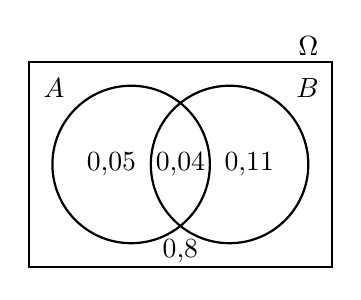
\begin{tikzpicture}[thick,
            set/.style = {circle,
                        minimum size = 2cm,
                        fill=white}]
            \draw [draw=black] (-1.3,-1.3) rectangle (2.55,1.3);
            % Set A
            \node[set,label={135:$A$}] (A) at (0,0) {};
            % Set B
            \node[set,label={45:$B$}] (B) at (1.25,0) {};
            % Circles outline
            \draw (0,0) circle(1cm);
            \draw (1.25,0) circle(1cm);
            % Set intersection label
            \node at (0.625,0) {0,04};
            \node at (-0.25,0) {0,05};
            \node at (1.5,0) {0,11};
            \node at (0.625,-1.1) {0,8};
            \node at (2.25,1.5) {$\Omega$};
        \end{tikzpicture}
    \end{center}
    Para saber $P(A^c\cup B^c)$, hay que sumar las probabilidades en naranja:
    \begin{center}
        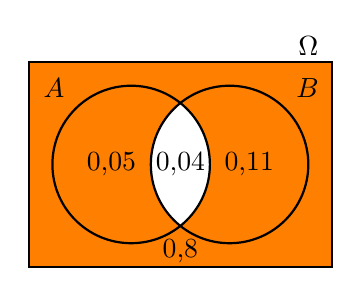
\begin{tikzpicture}[thick,
            set/.style = {circle,
                        minimum size = 2cm}]
            \fill[orange] (-1.3,-1.3) rectangle (2.55,1.3);
            \begin{scope}
                \clip (0,0) circle (1);
                \clip (1.25,0) circle (1);
                \fill[white] (1.25,0) circle (1);
            \end{scope}
            
            \draw [draw=black] (-1.3,-1.3) rectangle (2.55,1.3);
            % Set A
            \node[set,label={135:$A$}] (A) at (0,0) {};
            % Set B
            \node[set,label={45:$B$}] (B) at (1.25,0) {};
            % Circles outline
            \draw (0,0) circle(1cm);
            \draw (1.25,0) circle(1cm);
            % Set intersection label
            \node at (0.625,0) {0,04};
            \node at (-0.25,0) {0,05};
            \node at (1.5,0) {0,11};
            \node at (0.625,-1.1) {0,8};
            \node at (2.25,1.5) {$\Omega$};
        \end{tikzpicture}
    \end{center}
    Para saber $P(A^c\cap B^c)$:
    \begin{center}
        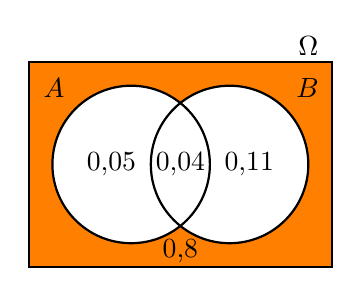
\begin{tikzpicture}[thick,
            set/.style = {circle,
                        minimum size = 2cm,
                        fill=white}]
            \fill[orange] (-1.3,-1.3) rectangle (2.55,1.3);
            \begin{scope}
                \clip (0,0) circle (1);
                \clip (1.25,0) circle (1);
                \fill[white] (-1.3,-1.3) rectangle (2.55,1.3);
            \end{scope}
            
            \draw [draw=black] (-1.3,-1.3) rectangle (2.55,1.3);
            % Set A
            \node[set,label={135:$A$}] (A) at (0,0) {};
            % Set B
            \node[set,label={45:$B$}] (B) at (1.25,0) {};
            % Circles outline
            \draw (0,0) circle(1cm);
            \draw (1.25,0) circle(1cm);
            % Set intersection label
            \node at (0.625,0) {0,04};
            \node at (-0.25,0) {0,05};
            \node at (1.5,0) {0,11};
            \node at (0.625,-1.1) {0,8};
            \node at (2.25,1.5) {$\Omega$};
        \end{tikzpicture}
    \end{center}
    Y finalmente, para $P(A\cap B^c):$
    \begin{center}
        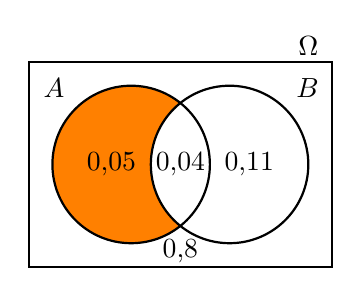
\begin{tikzpicture}[thick,
            set/.style = {circle,
                        minimum size = 2cm}]
            \fill[orange] (0,0) circle (1);
            \begin{scope}
                \clip (0,0) circle (1);
                \clip (1.25,0) circle (1);
                \fill[white] (0,0) circle (1);
            \end{scope}
            
            \draw [draw=black] (-1.3,-1.3) rectangle (2.55,1.3);
            % Set A
            \node[set,label={135:$A$}] (A) at (0,0) {};
            % Set B
            \node[set,label={45:$B$}] (B) at (1.25,0) {};
            % Circles outline
            \draw (0,0) circle(1cm);
            \draw (1.25,0) circle(1cm);
            % Set intersection label
            \node at (0.625,0) {0,04};
            \node at (-0.25,0) {0,05};
            \node at (1.5,0) {0,11};
            \node at (0.625,-1.1) {0,8};
            \node at (2.25,1.5) {$\Omega$};
        \end{tikzpicture}
    \end{center}
        \item Probar que $P(A\cap B)\geq P(A)+P(B)-1$
    \begin{align*}
        P(A\cap B)&=P(A)+P(B)-P(A\cup B)&&\text{Principio inclusión-exclusión}\\
        &\geq P(A)+P(B)-1&&P(A\cup B)\leq1\to -P(A\cup B)\geq -1
    \end{align*}
        \item Sean $E_1,\dots,E_n$ $n\geq2$, eventos cualesquiera de $S$.
    \begin{enumerate}
        \item Probar $P\left(\bigcup\limits_{i=1}^n E_i\right)\leq \sum\limits_{i=1}^nP(E_i)$\e\\
            Se define
            \begin{align*}
                B_1&=E_1\\
                B_2&=E_2-E_1\\
                B_3&=E_3-(E_1\cup E_2)\\
                \vdots\\
                B_n&=E_n-\left(\bigcup_{i=1}^{n-1}E_i\right)
            \end{align*}
            Sean $B_k,B_m, k>m$. Entonces $B_k=E_k-\left(\bigcup\limits_{i=1}^{k-1}E_i\right), B_m=E_m-\left(\bigcup\limits_{i=1}^{m-1}E_i\right)$
            \begin{align*}
                B_k\cap B_m&=E_k-\left(\bigcup_{i=1}^{k-1}E_i\right)\cap E_m-\left(\bigcup_{i=1}^{m-1}E_i\right)&&\text{Def}\\
                &=E_k\cap\left(\bigcup_{i=1}^{k-1}E_i\right)^c\cap E_m\cap\left(\bigcup_{i=1}^{m-1}E_i\right)^c&&\text{Resta}\\
                &=E_k\cap\left(\bigcap_{i=1}^{k-1}E_i^c\right)\cap E_m\cap\left(\bigcap_{i=1}^{m-1}E_i^c\right)&&\text{De Morgan}\\
                &=E_k\cap\left(\bigcap_{i=1}^{m-1}E_i^c\right)\cap\left(\bigcap_{i=m}^{k-1}E_i^c\right)\cap E_m\cap\left(\bigcap_{i=1}^{m-1}E_i^c\right)&&k>m\\
                &=E_k\cap\left(\bigcap_{i=1}^{m-1}E_i^c\right)\cap E_m^c\cap\left(\bigcap_{i=m+1}^{k-1}E_i^c\right)\cap E_m\cap\left(\bigcap_{i=1}^{m-1}E_i^c\right)\\
                &=\varnothing&&E_m^c\cap E_m\cap A=\varnothing\quad \forall A
            \end{align*}
            Si $m>k$, se pueden invertir los lugares y se llega al mismo resultado. Como consecuencia:
            \begin{equation}
                B_k\cap B_m=\varnothing\qquad\forall k\neq m
            \end{equation}
            Es decir, $B_k$ y $B_m$ son eventos independientes. Por otra parte, dado un $n$ arbitrario
            \[
                B_n=E_n-\left(\bigcup_{i=1}^{n-1}E_i\right)=E_n\cap\left(\bigcup_{i=1}^{n-1}E_i\right)^c\subseteq E_n
            \]
            \begin{equation}
                P(B_n)\leq P(E_n)
            \end{equation}
            Además, vemos que si $n=2$
            \begin{align*}
                \left(\bigcup_{i=1}^2 B_i\right)&=E_1\cup E_2-E_1\\
                &=E_1\cup E_2\cap E_1^c&&\text{Resta}\\
                &=(E_1\cup E_2)\cap(E_1\cup E_1^c)&&\text{Distributiva}\\
                &=(E_1\cup E_2)\cap\Omega\\
                &=E_1\cup E_2&&\text{Intersección con el universo}\\
                &=\left(\bigcup_{i=1}^2 E_i\right)
            \end{align*}
            Suponemos que funciona para un $n$ arbitrario y comprobamos para $n+1$
            \begin{align*}
                \bigcup_{i=1}^{n+1} B_i&=\left(\bigcup_{i=1}^{n} B_i\right)\cup B_{n+1}\\
                &=\left(\bigcup_{i=1}^{n} E_i\right)\cup B_{n+1}&&\text{Hipótesis Inductiva}\\
                &=\left(\bigcup_{i=1}^{n} E_i\right)\cup E_{n+1}-\left(\bigcup_{i=1}^{n} E_i\right)&&\text{Def }B_{n+1}\\
                &=\left(\bigcup_{i=1}^{n} E_i\right)\cup \left[E_{n+1}\cap\left(\bigcup_{i=1}^{n} E_i\right)^c\right]&&\text{Resta}\\
                &=\left[\left(\bigcup_{i=1}^{n} E_i\right)\cup E_{n+1}\right]\cap\left[\left(\bigcup_{i=1}^{n} E_i\right)\cup\left(\bigcup_{i=1}^{n} E_i\right)^c\right]&&\text{Distributiva}\\
                &=\left(\bigcup_{i=1}^{n+1} E_i\right)\cap \left[\left(\bigcup_{i=1}^{n} E_i\right)\cup\left(\bigcap_{i=1}^{n} E_i^c\right)\right]&&\text{De Morgan}\\
                &=\left(\bigcup_{i=1}^{n+1} E_i\right)\cap\left[\left(\left(\bigcup_{i=1}^{n} E_i\right)\cup E_1^c\right)\cap\dots\cap\left(\left(\bigcup_{i=1}^{n} E_i\right)\right)\cup E_n^c\right]&&\text{Distributiva}\\
                &=\left(\bigcup_{i=1}^{n+1} E_i\right)\cap\left[\Omega\cap\dots\cap\Omega\right]&&\text{En el término }j:E_j\cup E_j^c=\Omega\\
                &=\bigcup_{i=1}^{n+1} E_i&&\text{Intersección universo}
            \end{align*}
            Por lo tanto
            \begin{equation}
                \bigcup_{i=1}^{n} E_i=\bigcup_{i=1}^{n} B_i\qquad\forall n
            \end{equation}
            Con esto podemos ver que
            \begin{align*}
                P\left(\bigcup\limits_{i=1}^n E_i\right)&=P\left(\bigcup\limits_{i=1}^n B_i\right)&&\text{Por 3}\\
                &=\sum_{i=1}^nP(B_i)&&\text{Por 1}\\
                &\leq \sum\limits_{i=1}^nP(E_i)&&\text{Por 2}
            \end{align*}
        \item Probar que si cada $E_i$ es un evento casi seguro (es decir que $P(E_i)=1$), entonces $E_1\cap\dots\cap E_n$ es un evento casi seguro.\e\\
            Está en la teoría.
    \end{enumerate}
        \item Un sistema de control está formado por 10 componentes. La falla de cualquiera de ellos provoca la del sistema. Se sabe que la probabilidad de falla de cada componente es $<0.0002$. Probar que la probabilidad de que el sistema funcione es $>0.998$.\e\\
    $F=$"El sistema funciona"\\
    Se sabe que\[P(F)=1-P(F^c)=1-P(\text{el sistema no funciona})\]
    Para que el sistema no funcione, debe fallar por lo menos un componente, entonces si $A_i=$"el componente $i$ falla", tenemos que
    \[P(F)=1-P\left(\bigcup\limits_{i=1}^{10}A_i\right)\]
    Si suponemos que las fallas son independientes entre si:
    \[P(F)=1-\sum\limits_{i=1}^{10}P(A_i)\]
    Como $P(A_i)<0.0002\to-P(A_i)>0.0002$, por lo tanto
    \[P(F)>1-10\cdot0.0002\to P(F)>0.998\]
        \item Dados dos eventos $A$ y $B$, mostrar que la probabilidad de que ocurran exactamente uno de ellos es $P(A)+P(B)-2P(A\cap B)$\e\\
    Para que ocurra solamente $A$, tiene que ocurrir $A$ y no $B$. Mientras que para que ocurra solamente $B$, debe ocurrir $B$ y no $A$. Se ve que son eventos disjuntos, entonces
    \begin{align*}
        P(A-B)+P(B-A)&=P(A-(A\cap B))+P(B-(B\cap A))\\
        &=P(A)-P(A\cap B)+P(B)-P(A\cap B)&&A\cap B\subset A,\quad A\cap B\subset B\\
        &=P(A)+P(B)-2P(A\cap B)
    \end{align*}
        \item Sabiendo que $A\subset B$ y $P(A\cup B)=p,P(A\cap B)=q$, calcular: $P(A),P(B)$ y $P(A^c\cap B)$
    \begin{center}
        $A\subset B\to P(A\cup B)=P(B)\to P(B)=p$\\
        $P(A\cup B)=P(A)+P(B)-P(A\cap B)\to P(A)=P(A\cup B)+P(A\cap B)-P(B)\to P(A)=q$\\
        $P(A^c\cap B)=P(B\cap A^c)=P(B-A)=P(B)-P(A)=p-q$
    \end{center}
        \item Supongamos que $P(A)=0,8$ y $P(B)=0,3$. ¿Es correcto decir que $A\cap B=\varnothing$?¿Por qué?
    \begin{align*}
        P(A\cap B)&=P(A)+P(B)-P(A\cup B)&&\text{Principio de inclusión-exclusión}\\
        &=1,1-P(A\cup B)\\
        &\geq 1,1-1&&P(A\cup B)\leq1\to -P(A\cup B)\geq -1\\
        &=0,1
    \end{align*}
    Por lo tanto, no es correcta la afirmación ya que $P(A\cap B)\geq 0,1$
        \item Supongamos que $P(A\cup B)=P(A)+P(B)$. ¿Puedo asegurar que $A\cap B=\varnothing$?
    \[P(A\cup B)=P(A)+P(B)-P(A\cap B)\]
    Entonces \[P(A\cap B)=0\]
    Y se sabe que \[P(A\cap B)=0 \Leftrightarrow A\cap B=\varnothing\]
    Por lo tanto, sí se puede asegurar la intersección vacía.
    \end{enumerate}
\end{document}